
\section{ソフトの構成}
本研究で開発したソフトは,多数の関数で構成されている.
ここからは,各関数を機能ごとに詳述する.

\subsection{外部データの読み込み部}
\subsubsection{read\_pos}\begin{lstlisting}[style=customRuby,basicstyle={\scriptsize\ttfamily}]
def read_pos(lines, init_line=8)
  lattice, atom, poscar = [],[],[]
  lines[2..4].each{|line| lattice << line.scanf("%f %f %f\n")  }
  lines[init_line..lines.length+1].each{|line| atom << line.scanf("%f %f %f\n") }

  atom.each{|i_atom|
    pos=[0.0,0.0,0.0,0.0]
    i_atom.each_with_index{|atom_j,j|
      lx,ly,lz=lattice[j]
      pos[0] += atom_j*lx
      pos[1] += atom_j*ly
      pos[2] += atom_j*lz
    }
    poscar << pos
  }
  return poscar
end
\end{lstlisting}
関数read\_posは,外部データをARGVで読み込んでいるファイルlinesを受け取って.配列に格納する機能を果たしている.
コードの3行目では,linesの2行目から4行目の値を読み込んで配列lattticeに格納しており,コードの4行目では,lines内の8行目から最後の行までの座標を読み込んで配列atomsに格納している.
6行目からは,配列atomsをeach文で繰り返し演算をおこない,その中で配列lattice内に格納された各座標をlx,ly,lzと定義している.
定義した格子の各座標と原子の各座標との積をとることで原子配列の座標をもとめ,その値を配列poscarに格納している.

原子座標ファイルPOSCAR\_2223において,配列poscarに格納された原子座標を以下の実行結果で示す.
各括弧内の数値は,左から順にx座標,y座標,z座標を表している.
\begin{lstlisting}[style=,basicstyle={\scriptsize\ttfamily}]
% ruby viewer.rb POSCAR_2223 POSCAR_2223_4
[5.75101295815, 0.0, 0.0]
[7.668017277916733, 0.6390014395849836, 2.020699977875]
[3.834008638383265, 0.6390014395849836, 2.020699977875]
[7.029015837611088, 2.556005758968566, 0.0]
[4.473010078688911, 2.556005758968566, 0.0]
[5.75101295815, 0.0, 4.04139995575]
[7.668017277916733, 0.6390014395849836, 6.062099933625]
[3.834008638383265, 0.6390014395849836, 6.062099933625]
[7.029015837611088, 2.556005758968566, 4.04139995575]
[4.473010078688911, 2.556005758968566, 4.04139995575]
[6.390014398455645, 4.473010078352149, 2.020699977875]
[5.112011517844354, 4.473010078352149, 2.020699977875]
[6.390014398455645, 4.473010078352149, 6.062099933625]
[5.112011517844354, 4.473010078352149, 6.062099933625]
[9.585021596533265, 1.2780028797985992, 0.0]
[1.917004319766734, 1.2780028797985992, 0.0]
[8.946020157377822, 3.1950071991821813, 2.020699977875]
[2.556005758922177, 3.1950071991821813, 2.020699977875]
[0.0, 1.9170043193835826, 2.020699977875]
[10.863024475994353, 3.8340086387671652, 0.0]
[0.6390014403056455, 3.8340086387671652, 0.0]
[9.585021596533265, 1.2780028797985992, 4.04139995575]
[1.917004319766734, 1.2780028797985992, 4.04139995575]
[8.946020157377822, 3.1950071991821813, 6.062099933625]
[2.556005758922177, 3.1950071991821813, 6.062099933625]
[0.0, 1.9170043193835826, 6.062099933625]
[10.863024475994353, 3.8340086387671652, 4.04139995575]
[0.6390014403056455, 3.8340086387671652, 4.04139995575]
[8.307018717072177, 5.112011518565764, 0.0]
[3.1950071992278226, 5.112011518565764, 0.0]
[10.22402303683891, 5.751012958150748, 2.020699977875]
[1.2780028794610885, 5.751012958150748, 2.020699977875]
[8.307018717072177, 5.112011518565764, 4.04139995575]
[3.1950071992278226, 5.112011518565764, 4.04139995575]
[10.22402303683891, 5.751012958150748, 6.062099933625]
[1.2780028794610885, 5.751012958150748, 6.062099933625]
\end{lstlisting}
\subsection{原子座標の計算部}
\subsubsection{identical\_atoms}\begin{lstlisting}[style=customRuby,basicstyle={\scriptsize\ttfamily}]
def identical_atom(i_atom,j_atom)
  dist=0.0
  3.times{|i| dist += (i_atom[i]-j_atom[i])**2  }
  return true if Math.sqrt(dist)<0.5
  return false
end
\end{lstlisting}
関数identical\_atomsは,読み込んで計算した2つのPOSCARファイルに含まれる各々の原子座標の距離を求め,ある値を基準に大小比較をおこなう判定をしている.
コードの3行目で,ファイル内のある原子i\_atomともう片方のファイル内にある原子j\_atomの各座標の値を差分し,その値を2乗して加えることで原子間の距離を求めている.
その距離の値が,0.5より小さい値ならばtrue,そうでなければfalseと判定して返している.

\subsubsection{mk\_deleted\_atom}\begin{lstlisting}[style=customRuby,basicstyle={\scriptsize\ttfamily}]
def mk_deleted_atom
  mark=[]
  j_max = $pos_after.length
  $pos_before.each_with_index{|i_atom,i|
    update_num=0
    $pos_after.each_with_index{|j_atom,j|
      break if identical_atom(i_atom,j_atom)
      update_num = j
    }
    mark << $pos_before[i] if update_num==(j_max-1)
  }
  return mark
end
\end{lstlisting}
関数mk\_deleted\_atomは,原子削除をおこなう前後のPOSCARファイルを比較して削除された原子のみを別の配列に格納する機能を果たしている.
具体的に,コードの5行目で更新するための値update\_numを0と定め,2つのPOSCARファイルを演算しながら,原子間の距離を求める関数identical\_atomでtrueとして返されたものを配列markへ格納している.
POSCAR\_2223において,配列markに格納された原子座標を以下の実行結果で示す.
\begin{lstlisting}[style=,basicstyle={\scriptsize\ttfamily}]
% ruby viewer.rb POSCAR_2223 POSCAR_2223_4
[[6.390014398455645, 4.473010078352149, 2.020699977875, 0.0] 
[5.112011517844354, 4.473010078352149, 6.062099933625, 0.0] 
[10.863024475994353, 3.8340086387671652, 0.0, 0.0]
 [0.6390014403056455, 3.8340086387671652, 0.0, 0.0] 
[10.863024475994353, 3.8340086387671652, 4.04139995575, 0.0]]
\end{lstlisting}
\subsection{粒界原子の描画部}
\subsubsection{draw\_backcolor, draw\_axes}\begin{lstlisting}[style=customRuby,basicstyle={\scriptsize\ttfamily}]
def draw_backcolor
  $context.set_source_rgb(0.8, 0.8, 0.8)
  $context.rectangle(0, 0, $width, $height)
  $context.fill
end

def draw_axes
  $context.set_source_rgb(0, 0, 0)
  [[0,1],[1,0]].each{|line|
    x,y=line[0],line[1]
    [[0,0],[$cx,0],[0,$cy]].each{|c_x,c_y|
      $context.move_to($mv+c_x,$mv+c_y)
      $context.line_to($mv+c_x+x*$scale,$mv+c_y+y*$scale)
      $context.stroke
    }
  }
end
\end{lstlisting}
関数draw\_backcolorは,原子配列の背景を描画しており,原子配列を表示する画面のサイズを明確にするために挿入されている.
また,関数draw\_axesは,原子配列における縦軸と横軸を描画しており,コードの11行目にて3つ平面に必要な軸をまとめて出力できるようにしている.

\subsubsection{open\_circle}\begin{lstlisting}[style=customRuby,basicstyle={\scriptsize\ttfamily}]
def open_circle
  z_layer=[]
  layer_max, layer_min = $pos_max[2], 0.0
  bound=(layer_max - layer_min )/($denominator-1)
  num,j = layer_min, 0
  $diff = 0.15
  while num <= layer_max do
    z_layer[j] = num
    num += bound
    j += 1
  end
  return z_layer
end
\end{lstlisting}
関数open\_circleは,白抜きする層の座標を計算して配列に格納している.
コードの3行目に記述されたlayer\_maxは,関数find\_maxで得た原子のz座標の最大値を取っており,layer\_minはz座標の最小値として初期値0を与えている.
その直後に挿入されているboundは,各層の倍数値を取っている.
この倍数値は,z座標の最大値と最小値の差をとり,差分した数値を関数main\_drawで読み込んだ分母値denominatorで割ることにより値を得ている.
コードの7行目では,layer\_minからlayer\_maxまでの範囲で倍数値boundを加算させていき,加えていった各数値を配列z\_layerに格納している.
また,コード内に挿入されているdiffは,関数draw\_each\_planeにて白抜きする原子座標の近似値をさす.

\subsubsection{pos\_y}\begin{lstlisting}[style=customRuby,basicstyle={\scriptsize\ttfamily}]
def pos_y(pos, c_y, index, select)
  dy = select == 0 ? pos[index] : $pos_max[index]-pos[index]
  return $mv+c_y+$adjust*dy
end
\end{lstlisting}
関数pos\_yでは,x−y平面のy軸を逆転させる計算をおこない.描画する原子のy座標を返している.
具体的に,関数draw\_each\_planeの中のselで,描画する平面を識別した結果をもらい,x−y平面ならば,関数find\_maxにより得たy座標の最大値から各y座標を差分し,その値をdyへ与えている.
x−y平面以外の平面ならば,最大値からの差分を取らずにそのままの値を返している.

\subsubsection{draw\_each\_plane}\begin{lstlisting}[style=customRuby,basicstyle={\scriptsize\ttfamily}]
def draw_each_plane(ind_1,ind_2,c_x,c_y)
  rr = 2
  sel = (ind_1==0 and ind_2==1)? 1 : 0
  [[$deleted_atoms,[1,0,0],rr*1.3],[$pos_after,[0,0,1],rr]].each{|atoms_color|
    $context.set_source_rgb(atoms_color[1])
    radius = atoms_color[2]
    atoms_color[0].each{|pos|
      if $numerator == 0 then
        $context.circle($mv+c_x+$adjust*pos[ind_1],pos_y(pos,c_y,ind_2,sel), radius)
        $context.fill
      else
        if pos[2] < open_circle[$numerator-1]+$diff and open_circle[$numerator-1] - $diff < pos[2] then
          $context.circle($mv+c_x+$adjust*pos[ind_1],pos_y(pos,c_y,ind_2,sel), radius*1.7)
          $context.stroke
          $context.set_line_width(0.5)
        else
          $context.circle($mv+c_x+$adjust*pos[ind_1],pos_y(pos,c_y,ind_2,sel), radius)
          $context.fill
        end
      end
    }
  }

  if $pos_before.size==$pos_after.size
    $context.set_source_rgb(0, 0.8, 0)
    (0..$pos_before.length-1).each{|i|
      $context.move_to($mv+c_x+$adjust*$pos_before[i][ind_1],pos_y($pos_before[i],c_y,ind_2,sel))
      $context.line_to($mv+c_x+$adjust*$pos_after[i][ind_1],pos_y($pos_after[i],c_y,ind_2,sel))
      $context.stroke
    }
  end
end
\end{lstlisting}
関数draw\_each\_planeでは,描画する原子の位置,色,大きさを決定し,白抜き処理の判定をおこなっている.
コードの2行目にある値rrは,原子の半径値を示している.
4行目から,atoms\_colorの配列を組んで削除の有無により原子の色と大きさを変えて描画するようにしている.
また,8行目からは,原子の白抜き処理を判定している.具体的に,分子値numeratorが0であるかを判定し,trueならば白抜きなしの原子配列を描画する.
分子値numeratorが0でない,すなわち指定した層の値がnumeratorに入力されているのならば,関数open\_circleで各層の値を格納しているz\_layerの配列番号を指定し,近似値diffで範囲を求め,指定した層の白抜き処理をおこなう.
さらに,24行目からは,読み込んだ2つの原子配列ファイルPOSCARのデータサイズを比較している.同じサイズであるならば,2つのファイルにおける各原子間の距離を線で表示するようにしている.

\subsubsection{draw\_atoms}\begin{lstlisting}[style=customRuby,basicstyle={\scriptsize\ttfamily}]
def draw_atoms
  draw_each_plane(0,1,0,0)    
  draw_each_plane(0,2,0,$cy)   
  draw_each_plane(1,2,$cx,$cy) 
end
\end{lstlisting}
関数draw\_atomsでは,関数draw\_each\_planeで決定された原子配列を三面図の規定位置にそれぞれ描画するようにしている.
具体的に,x−y平面を平面図として第二象限,x−z平面を正面図として第三象限,y−z平面を側面図として第四象限に出力させている.

\subsubsection{find\_max}\begin{lstlisting}[style=customRuby,basicstyle={\scriptsize\ttfamily}]
def find_max(pos)
  max = [0,0,0]
  [0,1,2].each{|ind|
    pos.length.times {|i| max[ind] = pos[i][ind] if max[ind] < pos[i][ind] }
  }
  return max
end
\end{lstlisting}
関数find\_maxは,原子の各座標の最大値を探索する機能を果たしている.
関数read\_posにて,原子のx座標,y座標,z座標をそれぞれpos[0],pos[1],pos[2]の中に格納しており,隣接する値を比較することで,各座標の最大値を探索し,配列maxに格納している.

\subsubsection{main\_draw}\begin{lstlisting}[style=customRuby,basicstyle={\scriptsize\ttfamily}]
def main_draw(file1,file2, layer, model_scale = 10)
  lines1 = File.readlines(file1)
  lines2 = File.readlines(file2)
  if layer != nil then
    tmp=layer.split('/')
    $numerator, $denominator = tmp[0].to_f,tmp[1].to_f
  else
    $numerator = 0
  end
  
  $pos_before, $pos_after = read_pos(lines1,8), read_pos(lines2,8)
  $deleted_atoms = mk_deleted_atom
  
  $pos_max=find_max($pos_before)
  $pos_max[0].ceil*10
  $width,$height = 300,200
  $cx,$cy = $width/2.0,$height/2.0
  $mv = 10
  $scale = 1000
  $adjust = $scale/($pos_max[0].ceil*model_scale)
  surface = Cairo::SVGSurface.new('view.svg', $width, $height)
  $context = Cairo::Context.new(surface)
  $context.set_line_width($line_width)
  draw_backcolor
  draw_axes
  draw_atoms
  surface.finish
end
\end{lstlisting}
関数main\_drawには,描画機能の基盤が設定されており,rcairoで描画処理の基本となるサーフェスとコンテキストを作成し,出力場所及び出力先の形式を定めている.
2,3行目のlinesには,読み込んだ各々の外部ファイルを格納しており,コードの4行目では,白抜きする層の値が入力されているかを判定している.
この判定がtrueならば,入力値を/で分別し,それぞれの数値を分子値numerator, 分母値denominatorとして与えている.
また,判定がfalseならば,numeratorに0を与えている.
11行目では,読み込んだ2つの原子配列ファイルを関数read\_posで計算し,作成した原子座標poscarをファイルごとに分類している.
具体的に,初めのファイルの方をpos\_before,他方をpos\_afterとしている.
width,及びheightは,出力するスクリーンの大きさを指定しており,18行目のmvは,出力全体を移動させるための値である.
これは,軸上に存在している原子がスクリーンから出てしまうのを防ぐために挿入されている.
その直後に挿入されているscale,adjustは,出力する軸,並びに原子の大きさである.

なお,プログラムの文末には以下のコードを記述している.
\begin{lstlisting}[style=customRuby,basicstyle={\scriptsize\ttfamily}]
model_scale = 1.0/0.12
$line_width = 1
main_draw(ARGV[0],ARGV[1], ARGV[2],model_scale)
\end{lstlisting}
model\_scale,line\_widthは,出力する画面に対して軸や原子の大きさを調整するための数値である.

\subsection{三面図による描画}
三面図は,立体を正面図,平面図,側面図の三方向からみて投影した図を展開したもので,立体の形状を2次元上で的確に表示することが出来る.
開発当初は,上面,正面,側面の配置をまったく気にせずに図\ref{fig:009}(a)のように配置していた.
しかし,三方向から描く各図の位置はJIS規格で厳密に定めされており,正面図を物体の最も代表的な面と決められている\cite{ThreeViewDrawing}.
その正面図の真上に平面図,正面図の真横に側面図を描くことで三面図が作成される.
そこで,図\ref{fig:009}(b)のとおり最終版では修正して配置している.

\begin{figure}[htbp]\begin{center}
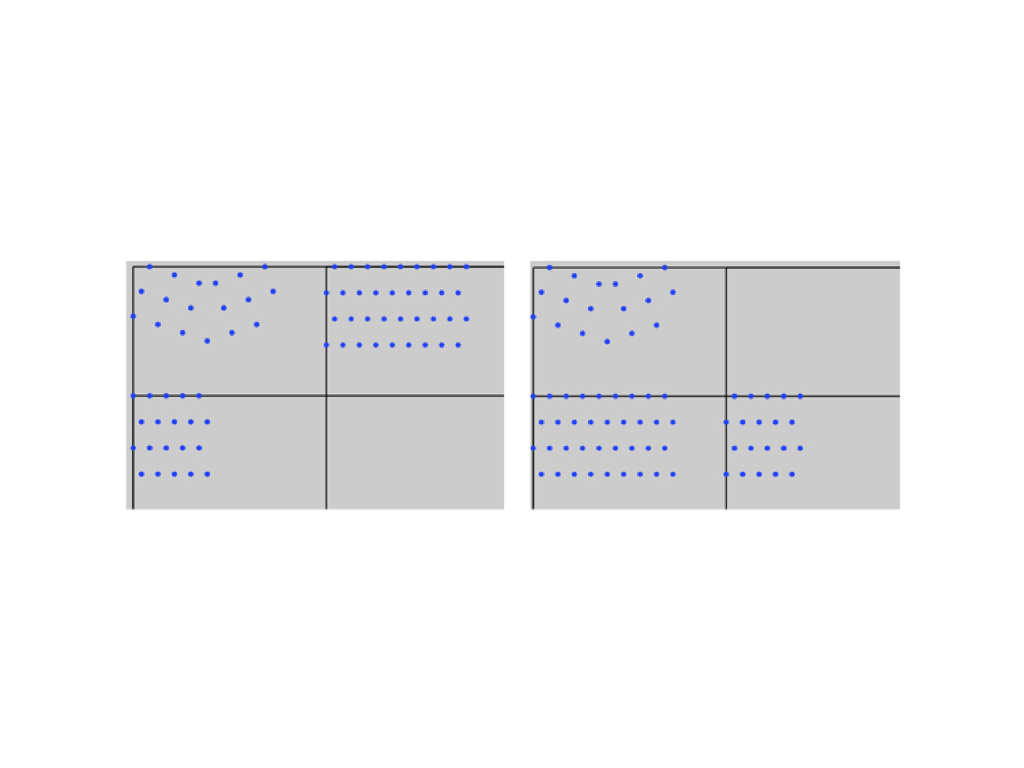
\includegraphics[width=12cm,bb= 0 0 937 753]{../figs/./boundary_narita.009.jpeg}
\caption{POSCAR\_2223を表示した三面図の(a)開発当初版と(b)最終版.}
\label{fig:009}
\label{default}\end{center}\end{figure}
